\documentclass[fleqn]{article}

\usepackage{polski}
\usepackage[utf8]{inputenc}
\usepackage[polish]{babel}
\usepackage{parskip}
\usepackage{icomma}
\usepackage[a4paper,includeheadfoot,margin=1.27cm]{geometry}
\usepackage{float}
\usepackage{graphicx}
\usepackage{amsmath}
\usepackage[hypcap=true]{subcaption}
\usepackage{xcolor}
\usepackage{transparent}
\usepackage{listings}
\usepackage[colorlinks=true, linkcolor=blue, pdfborder={0 0 0}]{hyperref}

\renewcommand\thesection{\arabic{section}.}
\renewcommand\thesubsection{\alph{subsection})}
\renewcommand\thesubsubsection{}
\newcommand\square[1]{
	\fcolorbox{black}{#1}{\rule{0pt}{6pt}\rule{6pt}{0pt}}
}

\brokenpenalty=1000
\clubpenalty=1000
\widowpenalty=1000

\lstdefinestyle{customc}{
	belowcaptionskip=1\baselineskip,
	breaklines=true,
	frame=L,
	xleftmargin=\parindent,
	language=C,
	showstringspaces=false,
	basicstyle=\footnotesize\ttfamily,
	keywordstyle=\bfseries\color{green!40!black},
	commentstyle=\itshape\color{purple!40!black},
	identifierstyle=\color{blue},
	stringstyle=\color{orange},
}


\title{TM -- Laboratorium 4. \\ \large Minutnik nastawiany przez \\ przytrzymanie przycisku + lub –}
\author{Krystian Chachuła \\ Dawid Gruszczyński \\ Marcin Skrzypkowski}

\begin{document}

\maketitle

\setcounter{page}{0}
\thispagestyle{empty}

\pagebreak

\setcounter{page}{1}

\section{Wstęp}

Naszym zadaniem na czwartym laboratorium było zaprojektowanie i zrealizowanie minutnika na platformie MSP430 w języku C. Czas miał być zadawany przez przyciski monostabilne, kolejnym założeniem było dołączenie dodatkowej funkcjonalności wzbogacającej działanie systemu oraz zapewniającej intuicyjne działanie.

Ostateczny układ składał się z następujących elementów:

\begin{itemize}
	\item \textbf{10\_PS1} (moduł zasilacza)
	\item \textbf{570\_MSP430F14x} (moduł mikrokontrolera Texas Instruments serii MSP430f14x lub F16x)
	\item \textbf{120\_IN8} (zestaw 8 monostabilnych wyłączników)
	\item \textbf{411\_WYS-DYN} (moduł wyświetlacza dynamicznego)
	\item \textbf{007\_TBD} (moduł głośnika ze wzmacniaczem)
\end{itemize}

\pagebreak

\section{Implementacja}

Do rozwiązania zadania podeszliśmy w sposób obiektowy. Projektowanie ropoczęliśmy od podziału zadania na mniejsze części, aby uzyskać większy komfort pracy i ułatwić orientację. Stowrzyliśmy więc struktury (klasy) służące do obsługi przycisków, wyświetlania symboli, podstawowych funkcji minutnika oraz odtwarzania melodii. Następnie zaplanowaliśmy ich podstawowe cechy w postaci pól oraz funkcjonalności w postaci metod bazujących na nich. Ogólną ideę rozwiązania przedstawia poniższy graf: % TODO tutaj chyba graf

\begin{figure}[H]
	\centering
	\begin{subfigure}[b]{0.49\textwidth}
		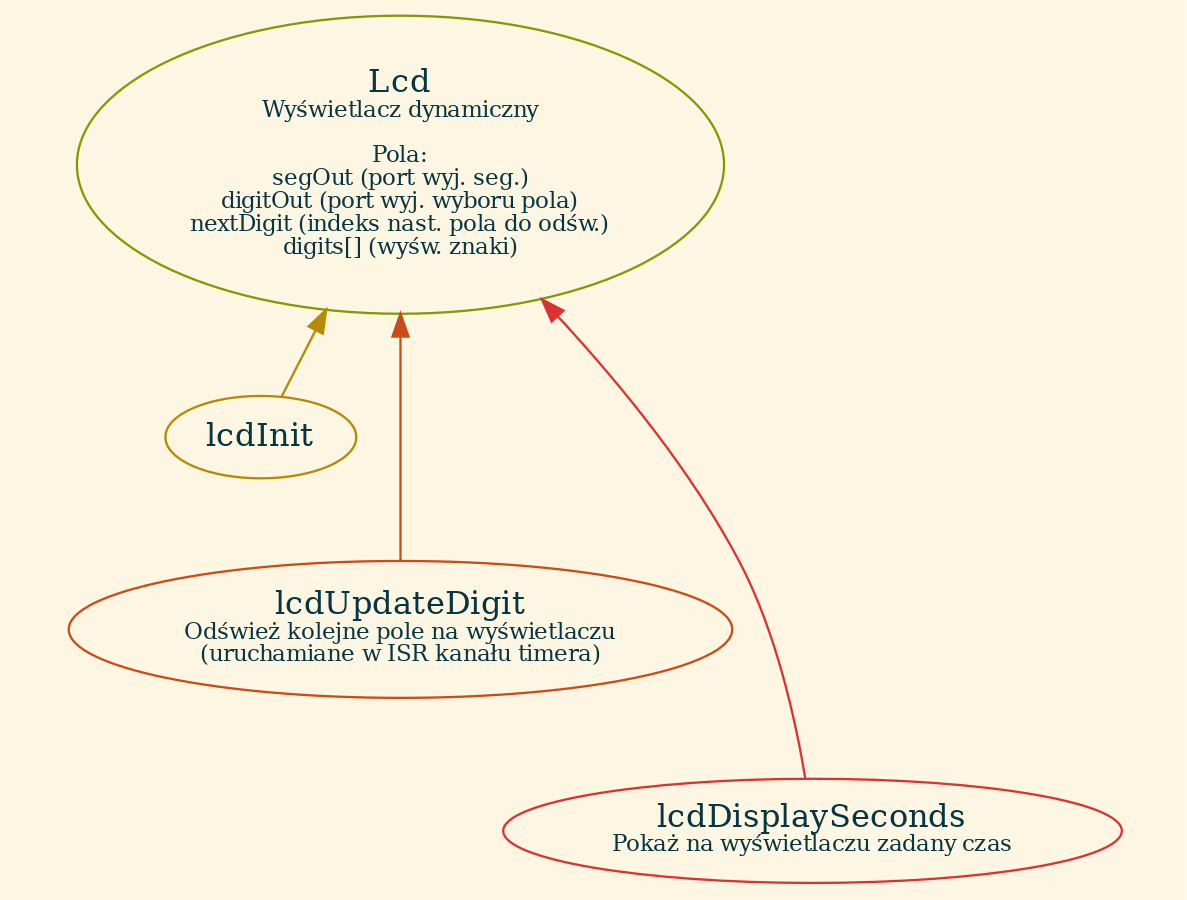
\includegraphics[width=\textwidth]{assets/g_lcd.png}
		\caption{Lcd}
	\end{subfigure}\hfill
	\begin{subfigure}[b]{0.49\textwidth}
		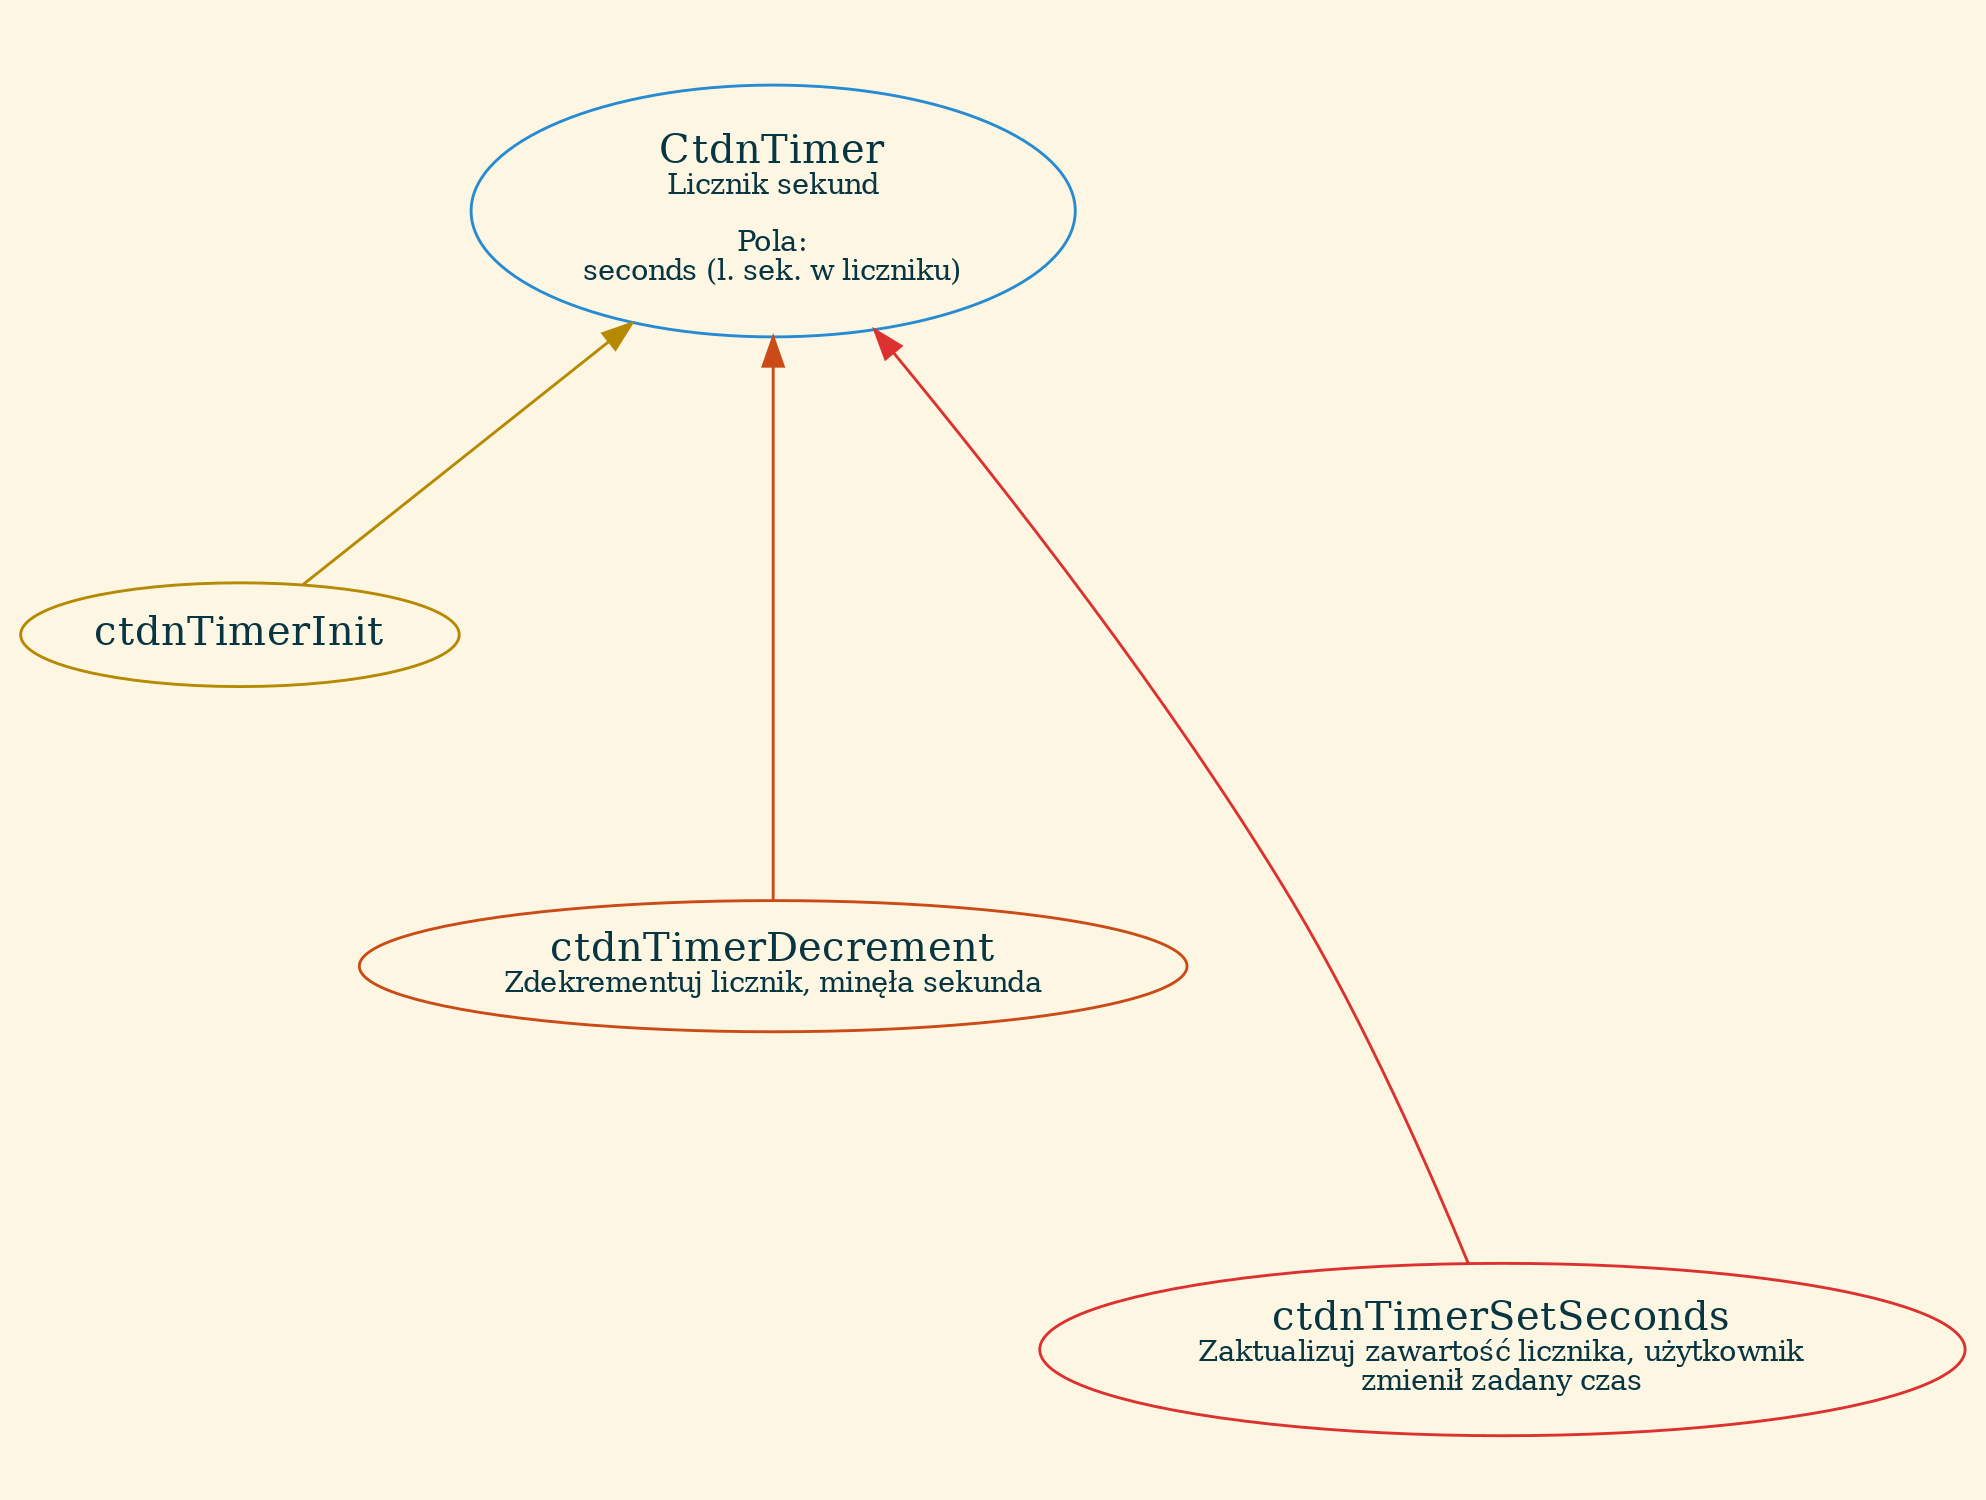
\includegraphics[width=\textwidth]{assets/g_ctdntimer.png}
		\caption{CtdnTimer}
	\end{subfigure}
	\par\bigskip
	\centering
	\begin{subfigure}[b]{0.49\textwidth}
		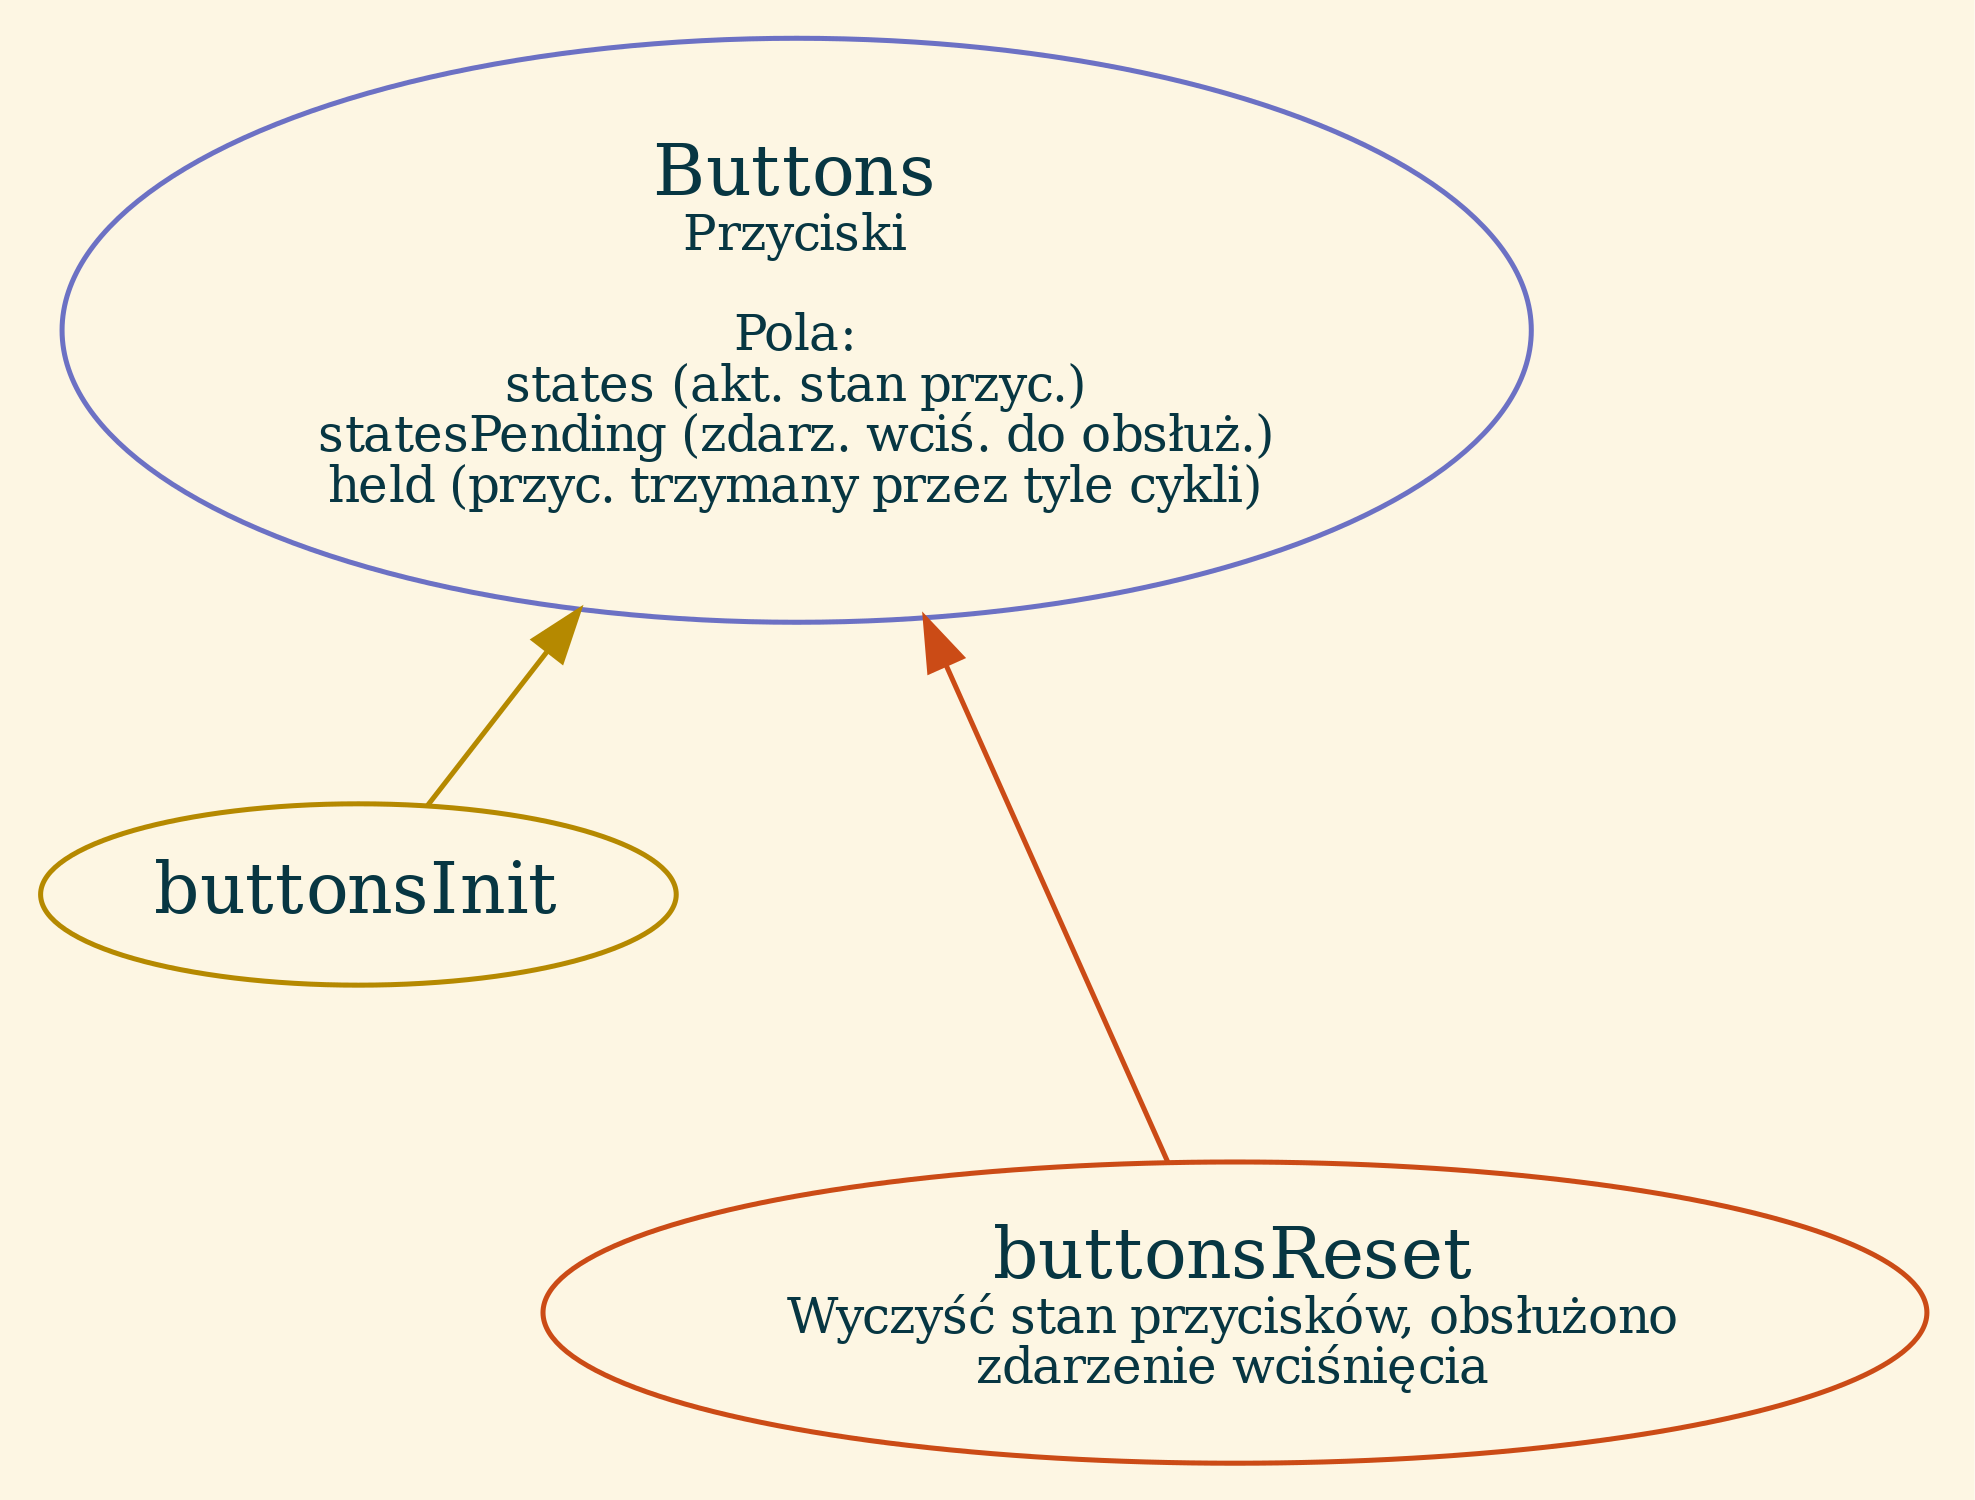
\includegraphics[width=\textwidth]{assets/g_buttons.png}
		\caption{Buttons}
	\end{subfigure}\hfill
	\begin{subfigure}[b]{0.49\textwidth}
		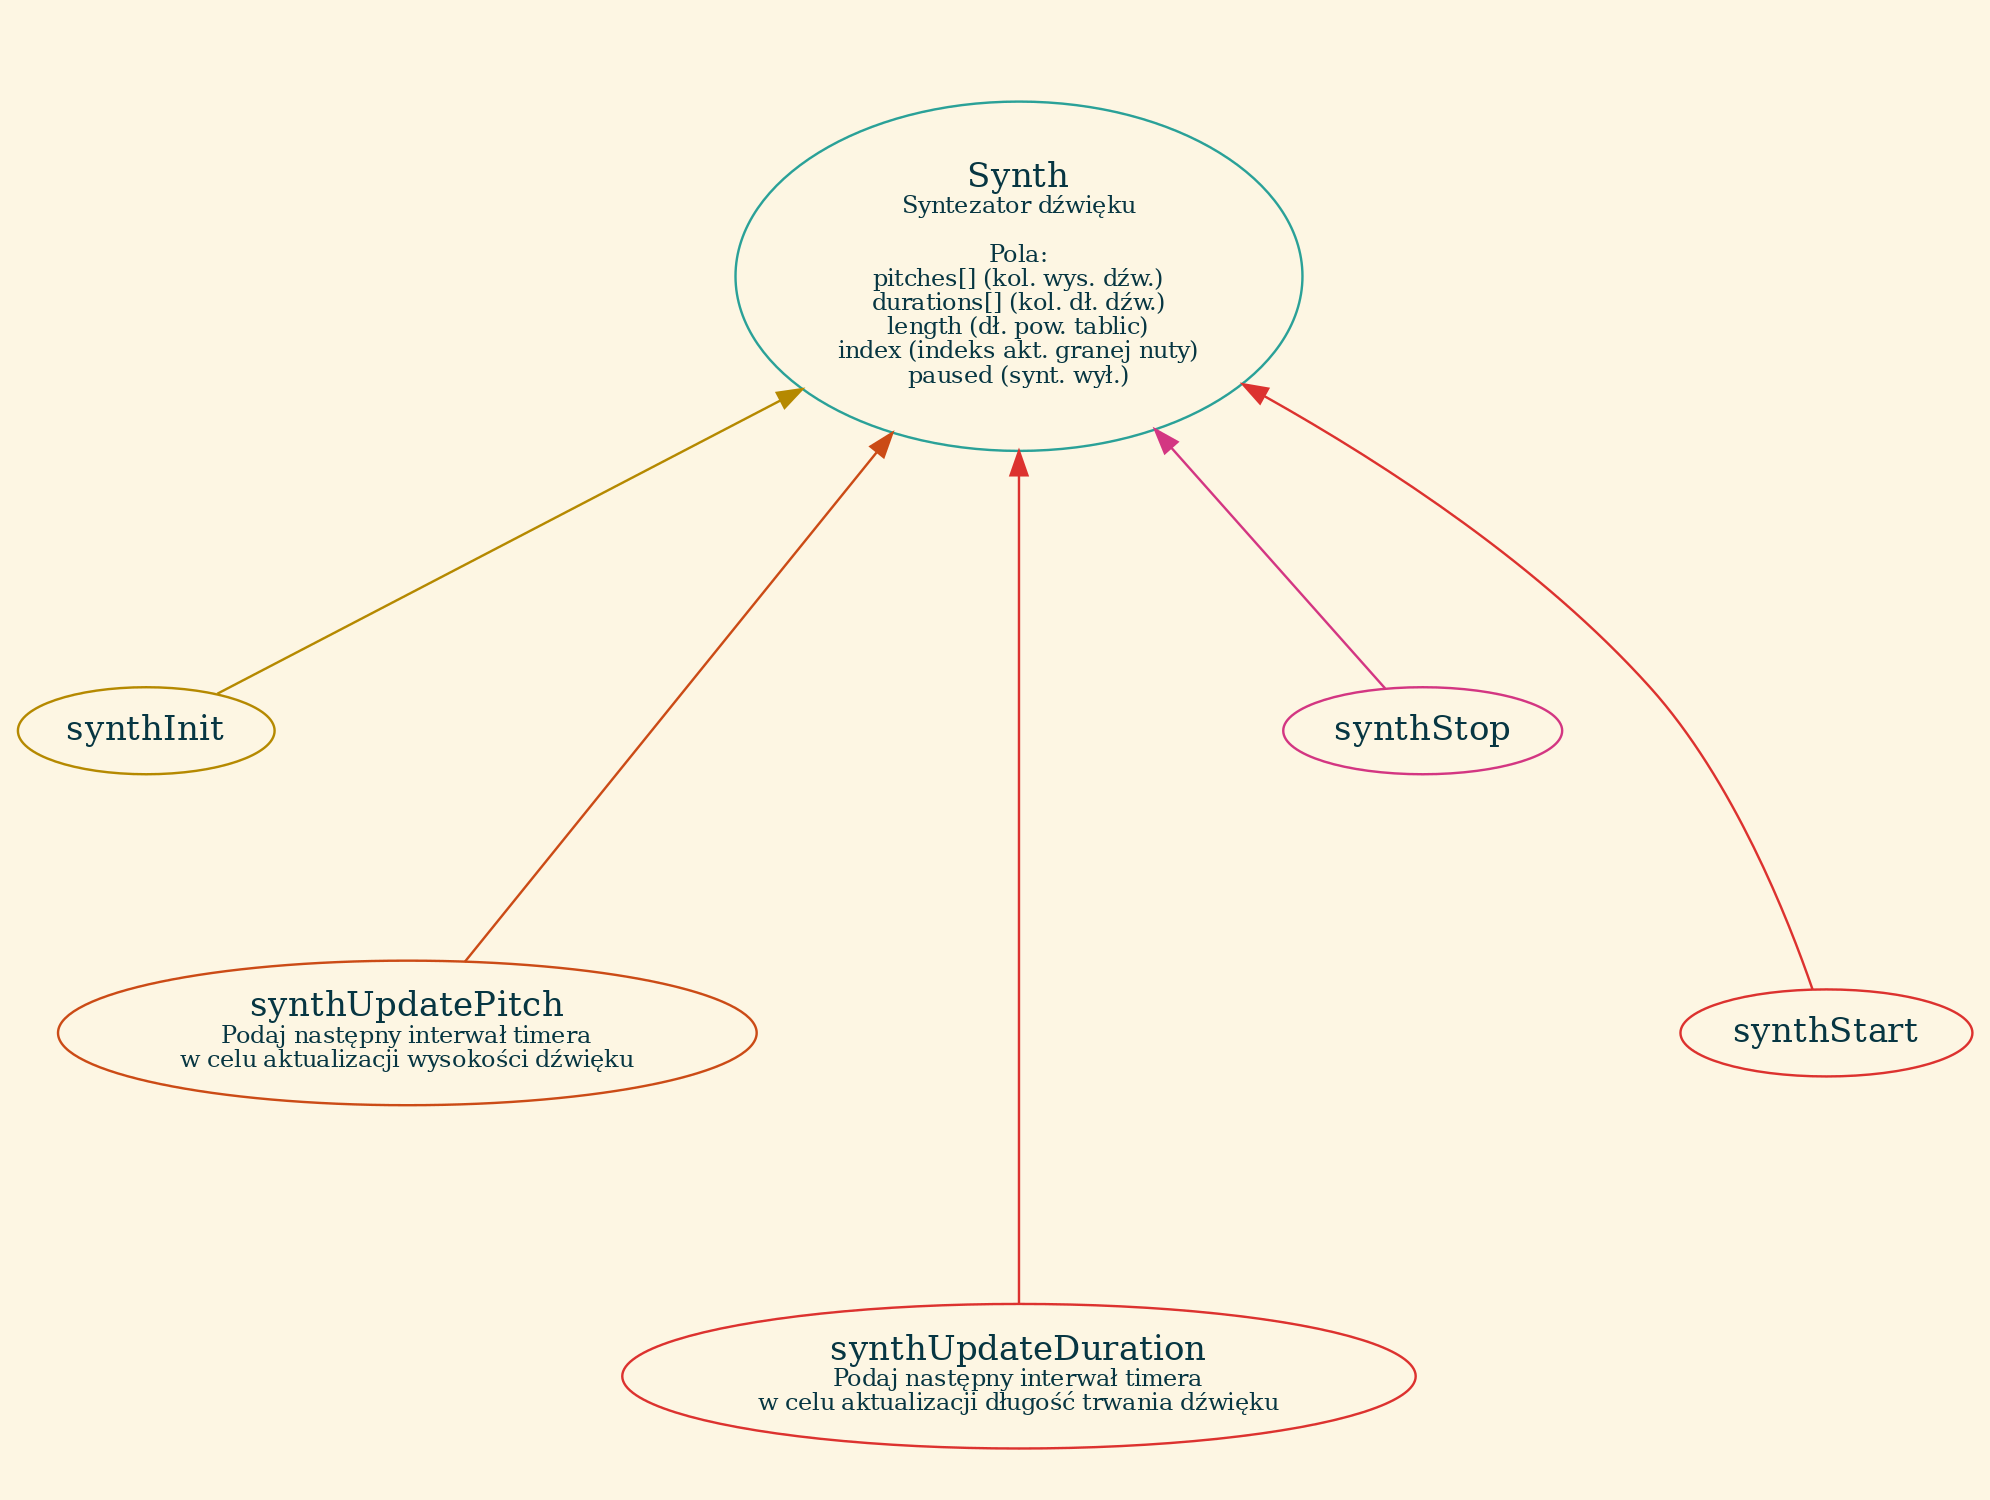
\includegraphics[width=\textwidth]{assets/g_synth.png}
		\caption{Synth}
	\end{subfigure}
	\caption{Klasy, ich metody oraz pola}
\end{figure}

\pagebreak

\section{Wyświetlanie}

Wyświetlacz dynamiczny, z którego korzystaliśmy w tym ćwiczeniu, ma możliwość wyświetlania tylko jednego symbolu na raz, przez co, w celu poprawnego wyświetlania zawartości minutnika, należy przełączać się pomiędzy kolejnymi znakami. Aby tego dokonać najpierw musieliśmy mieć możliwość manipulacji częstotliwością. Do odliczania jednej sekundy, która była potrzebna do wykonania zadania minutnika (założyliśmy dokładność jednej sekundy), wykorzystaliśmy zegar ACLK ustawiony na częstotliwość $32.768$ kHz. Natomiast do wywoływania cyklicznych przerwań wykorzystaliśmy główny kanał Timera A, a sam Timer skonfigurowaliśmy do trybu zliczania do wartości zawartej w rejestrze kanału. W celu sprawdzenia, czy wybrany przez nas sposób mierzenia czasu jest dopuszczalny, sprawdziliśmy częstotliwość generowania przerwań kanału na oscyloskopie. Poniżej znajdują się wyniki testów.

\begin{figure}[H]
	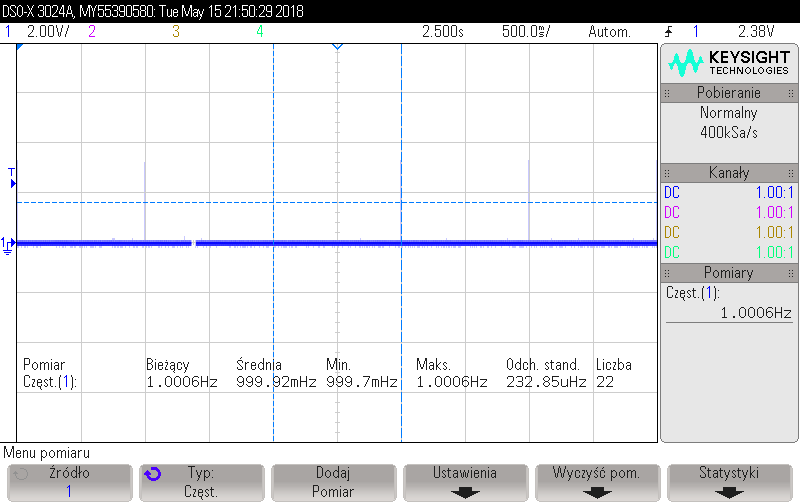
\includegraphics[width=\textwidth]{scope_1.png}
	\caption{Test odliczania jednej sekundy na wybranej przez nas częstotliwości $32.768 kHz$}
\end{figure}

Po 22 próbkach odchylenie standardowe od średniej równej $\frac{1}{1.0006\,Hz} = 0.9994\,s$ wynosiło $232.85$ $\mu$s. Stwierdziliśmy, że jest to wystarczająca dokładność do zrealizowania naszego zadania.

Ostateczna postać minutnika posiada pięć symboli, 2 cyfry odpowiedzialne za wyświetlanie minut, 2 cyfry odpowiedzialne za wyświetlanie sekund (maksymalną wartością możliwą do ustawienia $99:59$) oraz jeden symbol oznaczający tryb, w którym aktualnie znajduje się minutnik. W zależności od tego, w którym trybie znajduje się system, na ostatnim miejscu wyświetlana jest litera \textbf{t} (zliczanie) lub \textbf {c} (ustawianie).

Każdy znak ma być wyświetlany z częstotliwością co najmniej $60$ Hz, dlatego przełączanie pojedynczego symbolu następuje z częstotliwością $32768 / 60 / 5$ Hz. Program został napisany w taki sposób, aby można było wygodnie zmieniać częstotliwość odświeżania każdego z symboli.

\pagebreak

\section{Przyciski}

W końcowej wersji projektu zaimplementowaliśmy trzy przyciski, jeden do zwiększania wartości, od której minutnik zaczynał odliczanie, drugi do zmniejszania tej wartości, oraz dodany jako uzupełnienie funkcjonalności trzeci przycisk do natychmiastowego zerowania licznika. Mogą być one wpięte w dowolny port. Dodatkowo, aby zwiększyć komfort korzystania z systemu, wprowadziliśmy zwiększanie prędkości zmiany wartości minutnika proporcjonalnie z czasem trzymania przycisku. W razie przytrzymania dwóch przycisków jednocześnie, minutnik się zatrzymuje i czeka na puszczenie któregoś z nich. Również wciśnięcie dowolnego z nich powoduje zakończenie sygnalizowania, że minutnik doliczył do zera.

\section{Timery}

W systemie wykorzystujemy timer A do zliczania pełnych sekund i pięć kanałów z timera B do obsługi sygnału zliczenia do zera oraz obsługi wyświetlacza. Działanie timera A jest ustawione w tryp \textbf{UP} w celu umożliwienia zliczania wciąż do wartości $32768$, a więc pełnej sekundy. Timer B ustawiony został w tryb \textbf{continuous}, aby móc ustawić odpowiednie interwały potrzebne do obsługi debouncingu przycisków, odświeżania wyświetlacza oraz generowania sygnału zakończenia mierzenia czasu. Kanały odpowiadają kolejno za:
\begin{itemize}
	\item  \textbf{TACCTR0} zliczanie pojedynczych sekund
	\item  \textbf{TBCCTR0} częstotliwość odświeżania pojedynczego symbolu
	\item  \textbf{TBCCTR1} okres sprawdzania przycisków
	\item  \textbf{TBCCTR2} przyspieszanie zmiany wartości minutnika
	\item  \textbf{TBCCTR3} długość trwania dźwięku
	\item  \textbf{TBCCTR4} wysokość dźwięku
\end{itemize}

\section{Debouncing}
Wprowadzenie timerów pozwoliło nam na prostszą niż w poprzednim zadaniu implementację obsłgi przycisków. Debouncing odbywa się teraz przy pomocy kanału timera B, Za każdym razem gdy zostanie odliczony pewien interwał (długości BUTTON\_PERIOD), kanał TBCCR1 zgłasza przerwanie, w którym następuje sprawdzenie, czy któryś z przycisków jest wciśnięty. Jeśli tak, zostaje zinkrementowana wartośc licznika debouncingu. Dopiero gdy zostanie sprawdzonych odpowiednia ilość takich okresów pod rząd z wciśniętym przyciskiem, następuje jego obsługa.

\section{Usprawnienia oraz niezbędne modyfikacje projektu}

Minutnik wzbogaciliśmy o kilka dodatkowych funkcjonalności. Są to między innymi sygnalizacja trybu w jakim aktualnie się znajduje, zerowanie zawartości oddzielnym przyciskiem oraz odgrywanie melodii sygnalizujacej zakończenie odliczania.

Sygnalizacja trybu pracy odbywa się poprzez wyświetlanie na jednym z wyświetlaczy siedmiosegmentowych litery t gdy minutnik jest w trakcie odliczania lub litery c podczas gdy jest zatrzymany lub ustawiany jest czas zliczania.

Przycisk zerujący dodaliśmy w celu umożliwienia łatwego i szybkiego zerowania minutnika. Pozwala on także na wyłączenie alarmu sygnalizującego zakończenie zliczania.

Największym usprawnieniem minutnika jest odgrywanie melodii sygnalizującej zakończenie odliczania. Odbywa się to poprzez generację na wyjściu jednego z kanałów Timera B sygnału kwadratowego, a następnie podanie go na wejście wzmacniacza, który z kolei zasila głośnik wzmocnionym sygnałem. Do sterowania odgrywaniem melodii służy klasa Synth, która przechowuje informacje czasie trwania i częstotliwości kolejnych nut, natomiast za generację sygnału odpowiadają dwa kanały Timera B. Jeden z nich zajmuje się generowaniem sygnału kwadratowego, który podawany jest bezpośrednio na wzmacniacz. Drugi natomiast, jest odpowiedzialny za zmienianie aktualnie generowanej częstotliwości (wysokości dźwięku) po upłynięciu czasu trwania kolejnego dźwięku.

\pagebreak

Klasa Synth została napisana w ten sposób, aby stanowiła implementację uniwersalnego monofonicznego syntezatora dźwięku. Umożliwia to zaprogramowanie dowolnej sekwencji nut. Tłumaczenie zapisu nutowego na zapis zrozumiały dla syntezatora jest intuicyjny. Przyjmuje on listę par (wysokość, czas trwania). Program obłsuguje mnemoniczne nazwy dźwięków skali chromatycznej takie jak C, D, E, F itd. Aby otrzymać dźwięki takie jak np. Cis lub Ges należy najpierw odnaleźć dźwięk równoważny danemu, ale z końcówką -is, a następnie usunąć z nazwy literę i. Np. As $\rightarrow$ Gis $\rightarrow$ Gs (do programu należy wpisać Gs); Eis $\rightarrow$ F; Des $\rightarrow$ Cis $\rightarrow$ Cs. Można tego uniknąć poprzez wprowadzenie makr dla wszystkich dźwięków, ale przy tworzeniu tego projektu nie było takiej konieczności.

\begin{figure}[H]
	\centering
	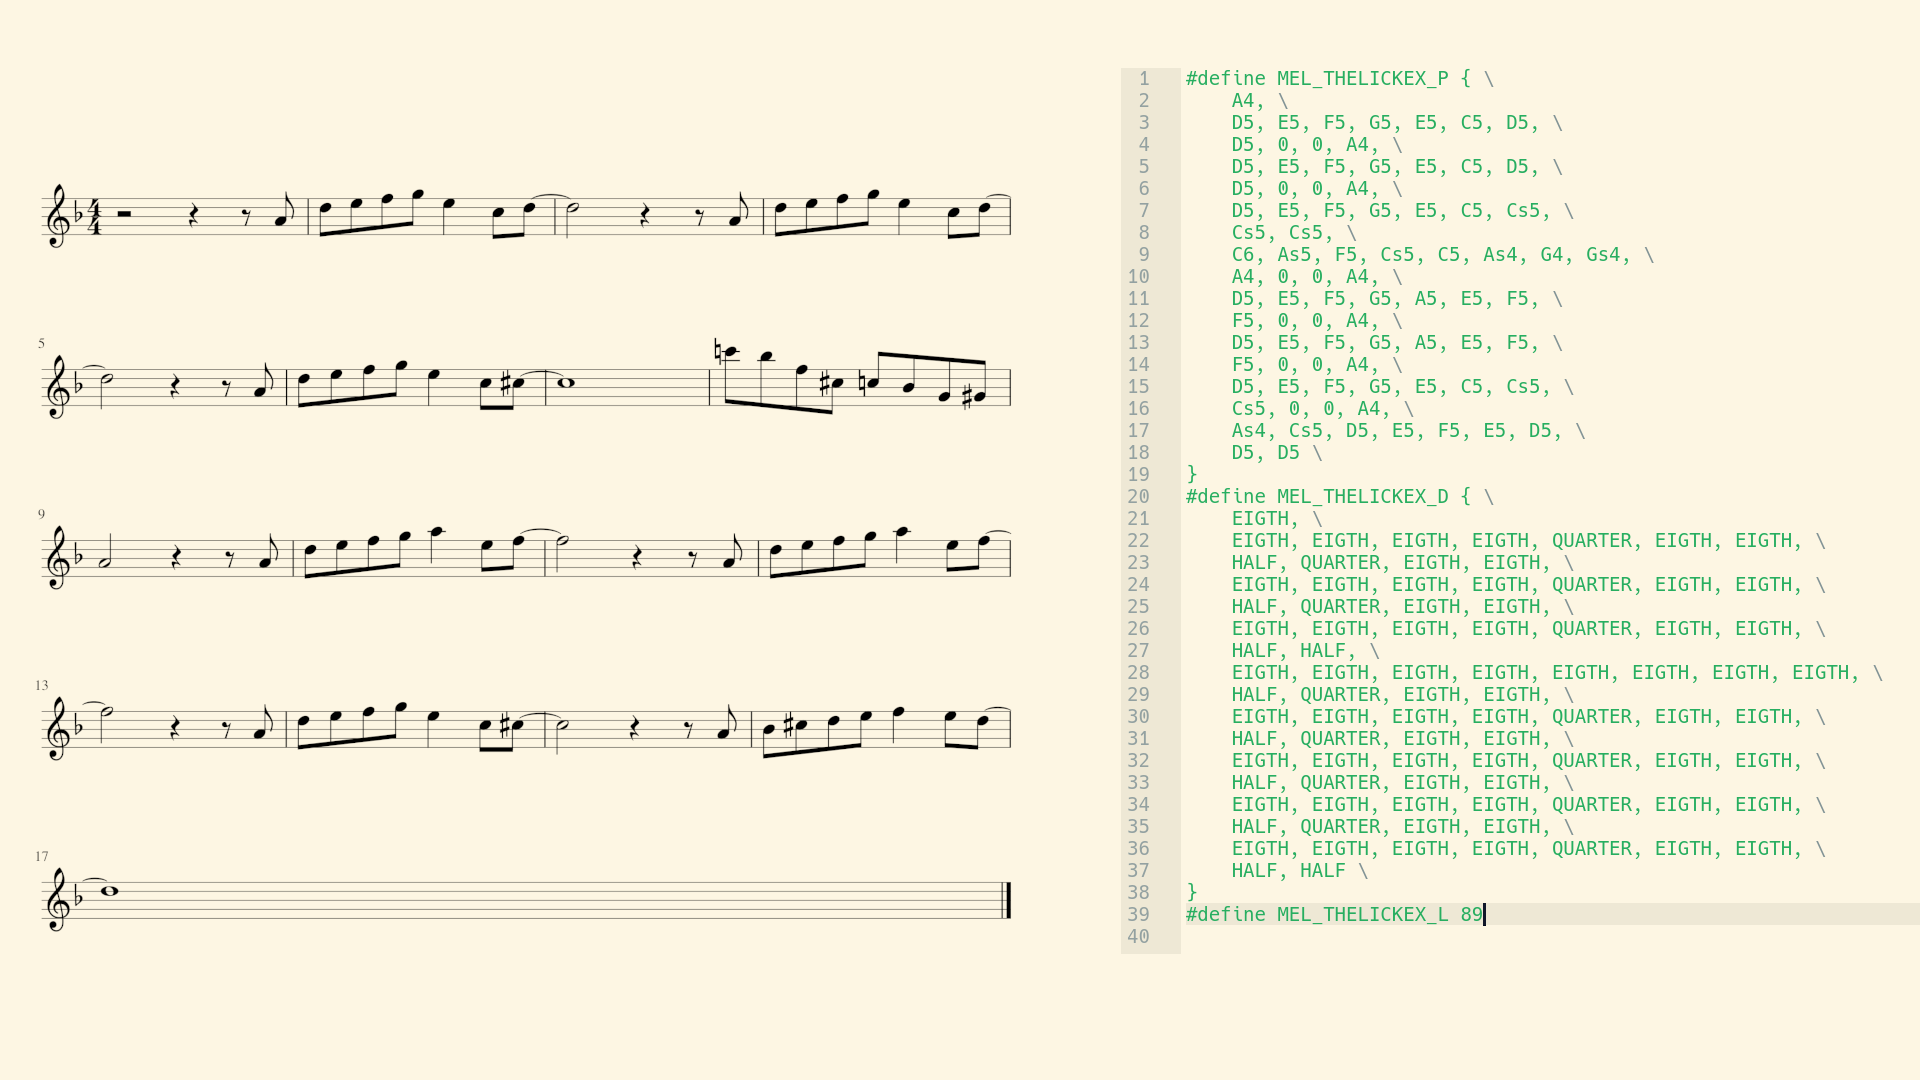
\includegraphics[width=\textwidth]{assets/synthdata.png}
	\caption{Przykład transkrypcji przetłumaczonej na potrzeby syntezatora}
\end{figure}

\section{Program}
\subsection{main.c}

\begin{minipage}[t]{.45\textwidth}
	\lstinputlisting[lastline=64, style=customc]{src/main.c}
\end{minipage}\hfill
\noindent\begin{minipage}[t]{.45\textwidth}
	\lstinputlisting[firstline=65, lastline=119, style=customc]{src/main.c}
\end{minipage}\hfill

\noindent\begin{minipage}[t]{.45\textwidth}
	\lstinputlisting[firstline=121, lastline=180, style=customc]{src/main.c}
\end{minipage}\hfill
\noindent\begin{minipage}[t]{.45\textwidth}
	\lstinputlisting[firstline=181, style=customc]{src/main.c}
	\subsection{Buttons}
	\subsubsection{Buttons.h}
	\lstinputlisting[style=customc]{src/Buttons.h}
	\subsubsection{Buttons.c}
	\lstinputlisting[style=customc]{src/Buttons.c}
\end{minipage}\hfill

\pagebreak

\subsection{Lcd}

\noindent\begin{minipage}[t]{.45\textwidth}
	\subsubsection{Lcd.h}
	\lstinputlisting[style=customc]{src/Lcd.h}
\end{minipage}\hfill
\noindent\begin{minipage}[t]{.45\textwidth}
	\subsubsection{Lcd.c}
	\lstinputlisting[style=customc]{src/Lcd.c}
\end{minipage}\hfill

\pagebreak

\noindent\begin{minipage}[t]{.45\textwidth}
\subsection{CtdnTimer}
\subsubsection{CtdnTimer.h}
\lstinputlisting[style=customc]{src/CtdnTimer.h}
\subsubsection{CtdnTimer.c}
\lstinputlisting[style=customc]{src/CtdnTimer.c}
\end{minipage}\hfill
\noindent\begin{minipage}[t]{.45\textwidth}
\subsection{melodies.h}
\lstinputlisting[style=customc]{src/melodies_slim.h}
\end{minipage}\hfill

\pagebreak

\section{Możliwości udoskonalenia systemu}
Możliwym udoskonaleniem minutnika byłoby przesyłanie melodii minutnika poprzez port szeregowy (na przykład za pomocą UART) w postaci MIDI. Umożliwiałoby to integrację z programami typu \textit{Digital Audio Workstation}, co z kolei zapewniałoby funkcjonalność minutnika jako pełnoprawnego syntezatora sprzętowego. Dodatkowo, używając \textbf{Przetwornika cyfrowo-analogowego} wbudowanego w MSP430. Syntezator mógłby generować różne typy przebiegów, aby osiągać rożne brzmienia. Ograniczeniem byłyby w tym przypadku jedynie jego dwunastobitowość oraz rozmiar pamięci do przechowywania tablic wartości sygnału.

\end{document}
\grid
